\documentclass[12pt]{article}
\usepackage[margin=1in]{geometry}
\usepackage{amsmath}
\usepackage{booktabs}
\usepackage{graphicx}
\usepackage{float}
\usepackage{caption}
\usepackage{enumitem}
\usepackage{hyperref}
\usepackage{cite}
\usepackage{multicol}
\usepackage{tabularx}
\usepackage{makecell}
\usepackage{amssymb}



\title{\textbf{Group Project Report}\\
\large Introduction to Probability and Statistics\\
BARC-MT 220-01 (Spring 2025)\\
Instructor: Pep Mateu}

\author{
    Alejandro De La Torre \\
    Brian Tobin \\
    Isabel Nold \\
    Matt Schwartz \\
    Meredith Kendall
}

\date{April 2025}

\begin{document}

\maketitle
\vspace{0.5em}
\begin{center}
\href{https://github.com/adelatorre2/adelatorre2-competition-group-project-mt220}{\texttt{GitHub Repository: Competition Group Project}}
\end{center}
\vspace{0.5em}

\vspace{0.5em}

\newpage
\tableofcontents
\newpage

\section*{Part 1: Theoretical vs. Empirical Probabilities}
\addcontentsline{toc}{section}{Part 1: Theoretical vs. Empirical Probabilities}

\subsection*{Objective}
\addcontentsline{toc}{subsection}{Objective}
To compare the theoretical probabilities of each Rock-Paper-Scissors (RPS) combination to the actual game data from \texttt{competition\_final.xls} \cite{mateu_competition_lastxlsx_2025}. Specifically, using methods found in \cite{montgomery_applied_2018}, we examine the probability of each possible hand matchup (e.g., Rock vs Paper, Scissors vs Rock, etc.) under two scenarios:
\begin{itemize}
    \item \textbf{Theoretical:} Assuming uniformly random play.
    \item \textbf{Empirical:} Based on observed play in the dataset.
\end{itemize}

\subsection*{Theoretical Probabilities}
\addcontentsline{toc}{subsection}{Theoretical Probabilities}
Assuming each hand is equally likely,
\[
P(\text{Rock}) = P(\text{Paper}) = P(\text{Scissors}) = \frac{1}{3}
\]
Thus, each pairing of Player 1 vs Player 2 has probability:
\[
P(i \text{ vs } j) = \frac{1}{3} \cdot \frac{1}{3} = \frac{1}{9} \approx 0.111
\]

For a full view of the expected probabilities across all matchups, see Table~\ref{tab:theoretical_matrix} in the Appendix.

\subsection*{Empirical Counts Matrix}
\addcontentsline{toc}{subsection}{Empirical Counts Matrix}
The actual number of times each pairing occurred in the dataset is displayed in Table~\ref{tab:empirical_counts} in the Appendix.

\subsection*{Empirical Proportions Matrix}
\addcontentsline{toc}{subsection}{Empirical Proportions Matrix}
To better compare observed results with theoretical expectations, we normalized the empirical counts into proportions. These are shown in Table~\ref{tab:empirical_proportions} in the Appendix.

\subsection*{Analysis and Comparison}
\addcontentsline{toc}{subsection}{Analysis and Comparison}
\begin{itemize}
    \item The theoretical matrix (Table~\ref{tab:theoretical_matrix}) is symmetric and uniform, reflecting the assumption of equally likely hand selection.
    \item The empirical data (Table~\ref{tab:empirical_counts} and Table~\ref{tab:empirical_proportions}) shows deviations from this uniformity, which is to be expected. Scissors, for instance, appears more frequently than expected in both play and matchups.
    \item The highest proportion is Scissors vs Scissors (0.150), suggesting a behavioral tendency toward Scissors or potential mimicry.
    \item Rock vs Rock (0.067) appears significantly less than expected, hinting at underuse of Rock.
\end{itemize}

The empirical play patterns deviate from random choice assumptions. This suggests either strategic adaptation, psychological preference, or game-learning behavior over time. On the subject of preference towards scissors, there exists a possibility that players anticipating the game googled: "best strategy in rock paper scissors" and got advice to randomize their hand, and since \href{https://www.fishersci.com/us/en/education-products/publications/headline-discoveries/2025/spring-summer/rock-paper-scissors-science.html#:~:text=In%20RPS%2C%20each%20option%20has,paper%2C%20and%2026%20percent%20scissors.}{rock is the most commonly played hand}, there must have been a perceived randomness in choosing to play scissors in any given match up \cite{northam_rock_2025}. Alternatively, with the knowledge that rock is the most common hand and that we typically played during the last few minutes of class, players could have opted to use a \href{https://wrpsa.com/the-worst-rock-paper-scissors-strategies/}{scissors-dominant, double exclusion strategy} in an effort to lose quickly to leave the class as soon as possible \cite{world_rock_paper_scissors_association_worst_2021}. Further analysis in later parts will investigate changes across rounds and player strategies.

\newpage

% Part 2
\section*{Part 2: Player Behavior in Early vs. Later Rounds}
\addcontentsline{toc}{section}{Part 2: Player Behavior in Early vs. Later Rounds}


\subsection*{Overview}
\addcontentsline{toc}{subsection}{Overview}
In this section, we analyze player behavior in different segments of the competition, specifically comparing the first two rounds of each game to the rest of the rounds. This includes an examination of the frequency of each hand (Rock, Paper, Scissors) used and the outcomes (Win, Loss, Tie) for each player across these segments.

\subsection*{Summary of All Hands Played}
\addcontentsline{toc}{subsection}{Summary of All Hands Played}
With guidance from \cite{sawitzki_computational_nodate
}, we begin by reporting the total number of times each player used Rock, Paper, or Scissors throughout the entire competition.

\begin{itemize}
    \item See Table~\ref{tab:overall_counts} in the Appendix for the full breakdown of overall throw counts.
\end{itemize}

\subsection*{First Two Rounds Analysis}
\addcontentsline{toc}{subsection}{First Two Rounds Analysis}
Next, we focus on the first two rounds of each game and count:

\begin{itemize}
    \item The number of wins, losses, and ties each player recorded (see Table~\ref{tab:first2_outcomes}).
    \item The number of times each player chose Rock, Paper, or Scissors (see Table~\ref{tab:first2_counts}).
\end{itemize}

\subsection*{Remaining Rounds Analysis}
\addcontentsline{toc}{subsection}{Remaining Rounds Analysis}
Then, we isolate all rounds \textbf{after} the first two in each game to determine:

\begin{itemize}
    \item The distribution of wins, losses, and ties (see Table~\ref{tab:rest_outcomes}).
    \item The hand selection frequencies (see Table~\ref{tab:rest_counts}).
\end{itemize}

\subsection*{Comparative Analysis and Discussion}
\addcontentsline{toc}{subsection}{Comparative Analysis and Discussion}
By contrasting the early-round data with later-round behavior, we can evaluate whether players adjusted their strategy as the game progressed. Some key questions we investigate include:

\begin{itemize}
    \item Do players tend to use Rock more often early in a match?
    \item Are tie rates higher in the early rounds than in the later ones?
    \item Do win/loss ratios shift as players adapt to their opponents?
\end{itemize}

\vspace{1em}

\noindent\textbf{Chi-Square Test of Strategy Shift}\\
To statistically evaluate whether players changed their strategy between the first two rounds and the remaining rounds, we ran a Chi-Square Test of Independence for each player. The null hypothesis was that the player’s proportion of Rock, Paper, and Scissors moves remained the same across both segments of play. The alternative hypothesis was that the distribution changed significantly between the two segments.

\begin{itemize}
    \item If the p-value was less than 0.05, we considered the result significant and concluded that the player likely adjusted their strategy.
    \item If the p-value was greater than or equal to 0.05, we concluded that the player likely maintained a consistent strategy.
\end{itemize}

\noindent A summary of each player’s p-value, test statistic, and significance determination is presented in Table~\ref{tab:strategy_shift} in the Appendix.

\vspace{1em}
\begin{figure}[H]
\centering
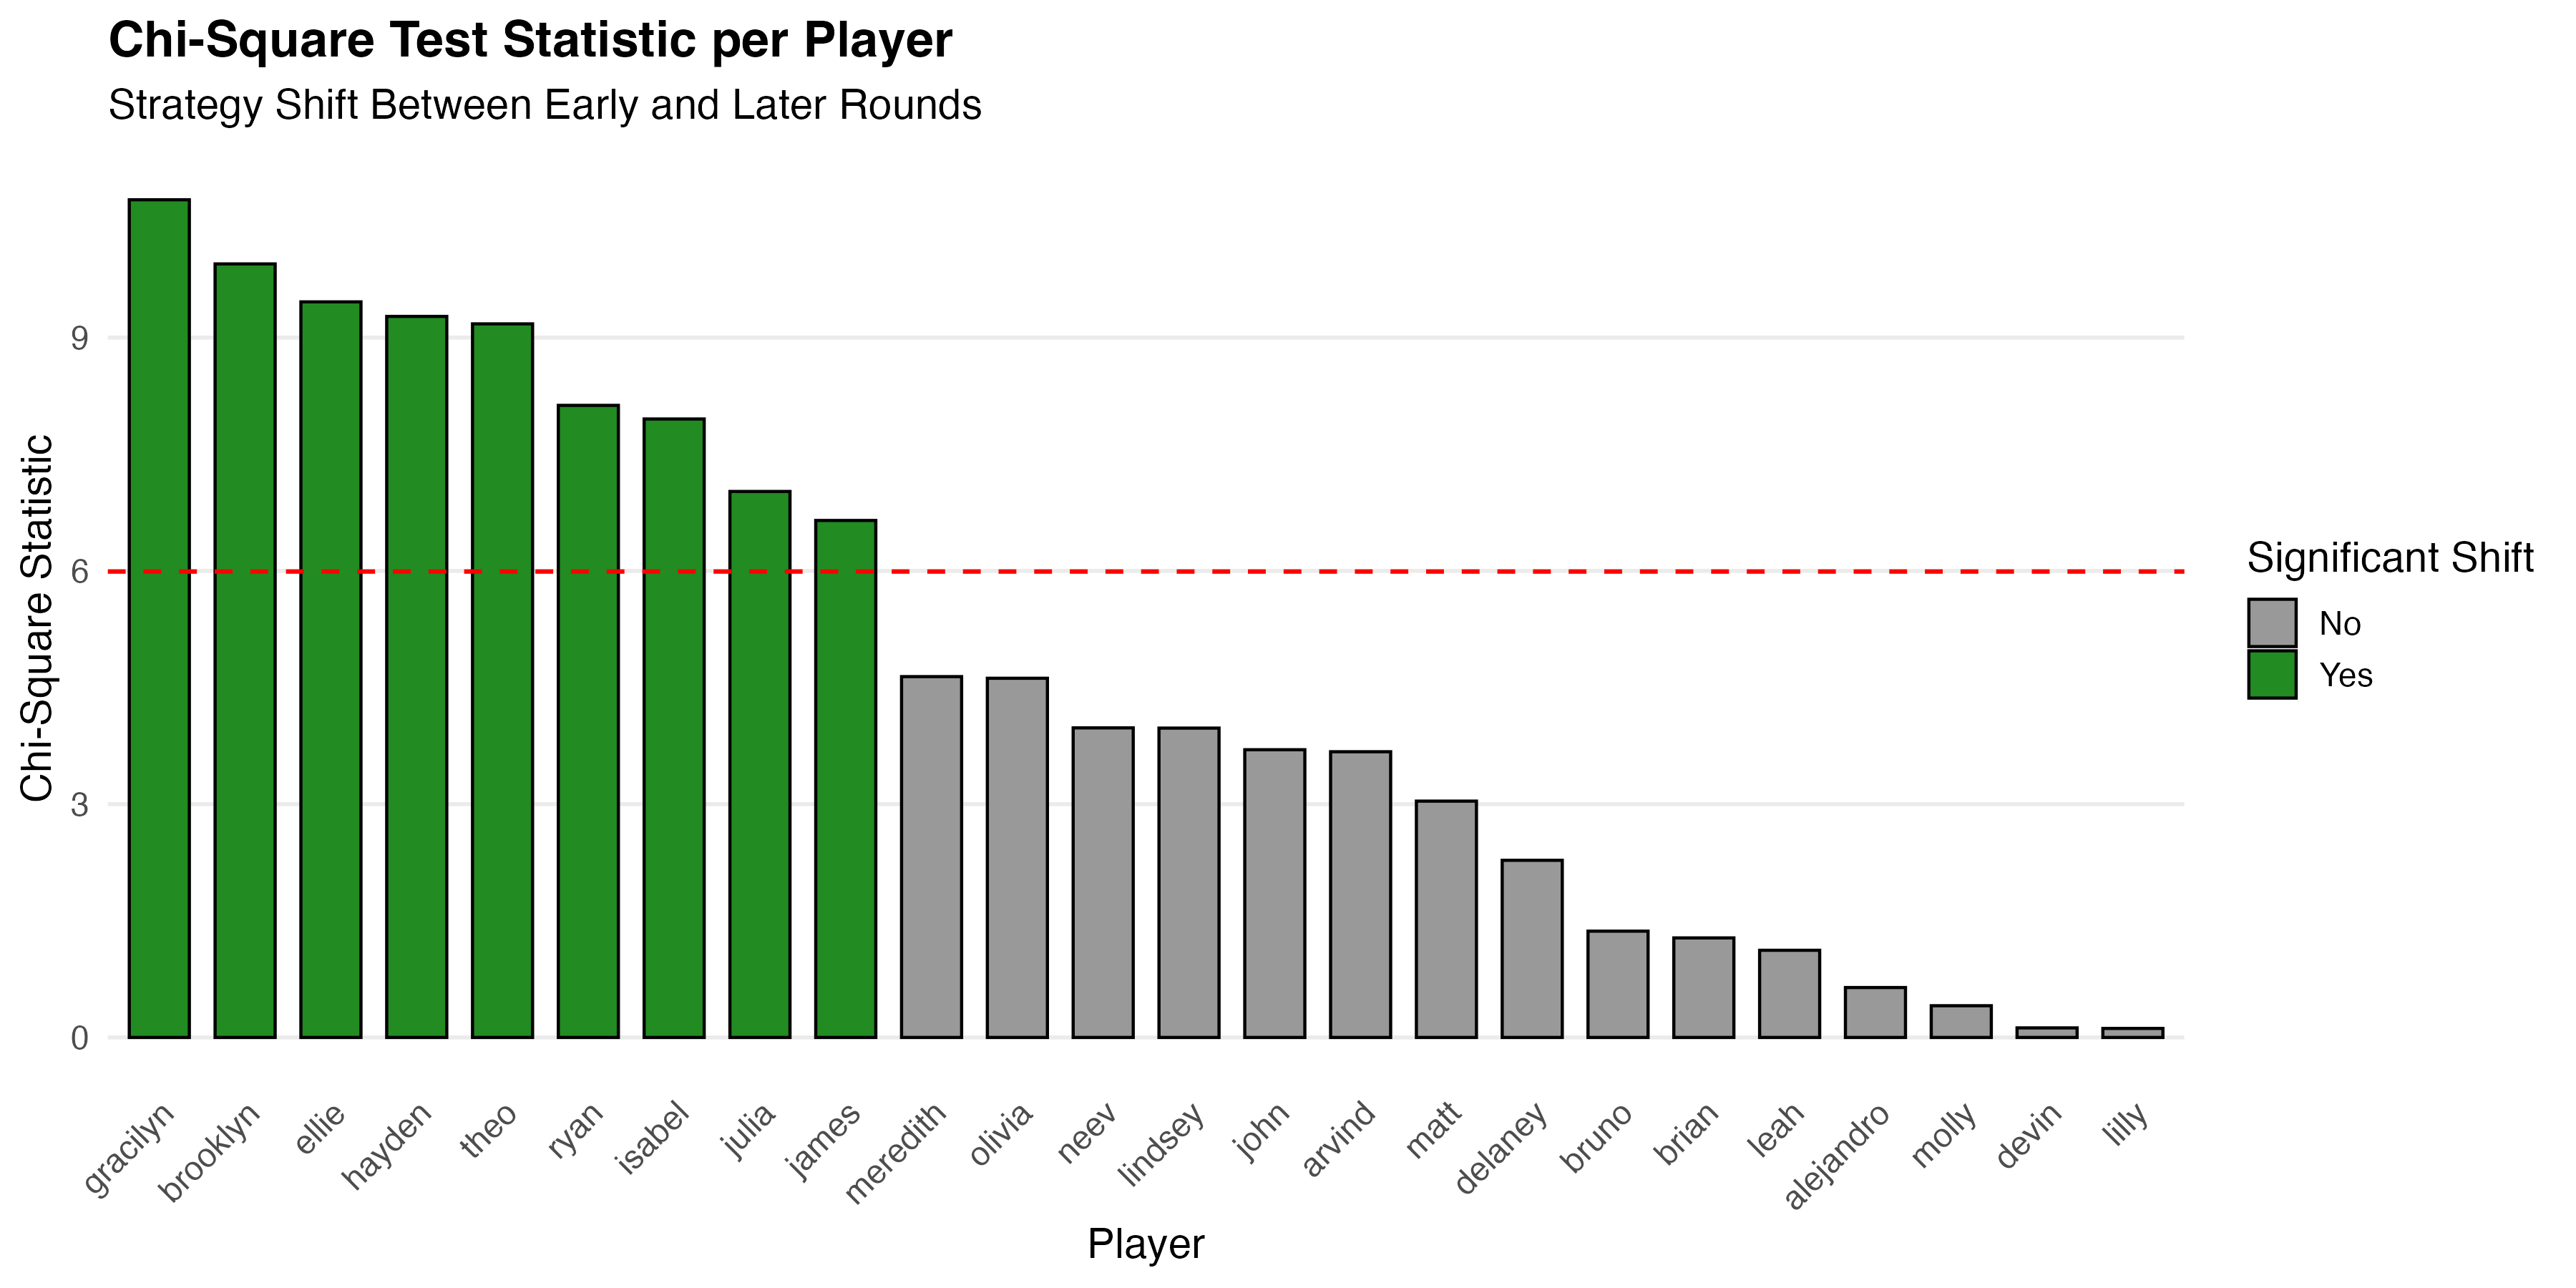
\includegraphics[width=0.8\textwidth]{figures/strategy_shift_chisq.png}
\caption{Chi-Square Test Statistic per Player (Strategy Shift Between Early and Later Rounds)}
\label{fig:strategy_shift_bar}
\end{figure}

\noindent\textbf{Interpretation of Chart:}\\
The bar chart above displays the Chi-Square test statistic for each player. Bars colored green indicate that the player's strategy changed significantly between early and later rounds ($p < 0.05$), while gray bars indicate no significant change. The red dashed line represents the critical value for the Chi-Square test with 2 degrees of freedom at the 0.05 significance level ($\approx 5.991$).

This visual makes it easy to quickly spot which players shifted strategies (i.e., changed the distribution of R/P/S hands) over time. For example, \texttt{gracilyn}, \texttt{brooklyn}, and \texttt{ellie} all scored above the threshold, indicating adaptive play. In contrast, players like \texttt{lilly}, \texttt{molly}, and \texttt{alejandro} remained more consistent in their hand selection.

\vspace{1.5cm}

\noindent\textbf{What This Chart Tells Us:}
\begin{itemize}
    \item It quantifies how much each player’s behavior changed between game segments.
    \item It highlights statistically significant changes in behavior, controlling for random variation.
    \item It provides a broad snapshot of adaptability across all players.
\end{itemize}

\noindent\textbf{What This Chart Does \emph{Not} Tell Us:}
\begin{itemize}
    \item It does not explain \textit{why} a player changed their strategy.
    \item It does not tell us \textit{how} they changed (e.g., more Paper? less Rock?).
    \item It does not assess the \textit{effectiveness} of any strategy shift.
\end{itemize}

\noindent\textbf{Takeaways:}
\begin{itemize}
    \item A significant number of players altered their strategy mid-game, suggesting they adapted based on experience, opponent behavior, or game state.
    \item Others stuck to a consistent strategy, which could reflect randomness, commitment to a fixed plan, or lack of strategic adjustment.
    \item This pattern reinforces the idea that RPS in a competitive classroom setting is more dynamic than purely random.
\end{itemize}

\newpage

% Part 3
\section*{Part 3: Standings and Strategy Analysis}
\addcontentsline{toc}{section}{Part 3: Standings and Strategy Analysis}

\subsection*{Final Standings}
\addcontentsline{toc}{subsection}{Final Standings}

To evaluate overall performance in the tournament, we used the number of game wins as the primary ranking criterion and resolved ties using the number of game losses as a tiebreaker. A game was defined as won once a player accumulated three round victories against an opponent.

The top five players were: Ellie (16W, 6L), Isabel (15W, 8L), Matt (14W, 9L), Brian (13W, 10L), and Hayden (13W, 10L). The bottom five were: Lilly (4W, 17L), Devin (5W, 15L), Bruno (6W, 15L), Meredith (9W, 14L), and Molly (9W, 14L). The full tournament ranking is summarized in Table~\ref{tab:total_game_results}, and the individual match performance of each player (i.e., the total number of round-level wins, losses, and draws) is reported in Table~\ref{tab:total_match_results}.

\subsection*{Interpretation of Groupmate Performance}
\addcontentsline{toc}{subsection}{Interpretation of Groupmate Performance}

To understand why our group members—Isabel, Matt, Brian, Alejandro, and Meredith—placed where they did, we analyzed their tournament results and hand selection behavior. Specifically, we examined their number of game wins and losses, most-used hand (Rock, Paper, or Scissors), and whether they significantly changed strategies between the first two rounds and the remainder of each game. These summary statistics are shown in Table~\ref{tab:groupmate_summary}.

Among our groupmates, only Isabel demonstrated a statistically significant shift in strategy over time (based on a chi-squared test with $\alpha = 0.05$), while the others showed no such evidence of change. Notably, three of the five relied most heavily on Scissors, with Matt favoring Rock and Meredith favoring Paper. This suggests that although the group’s play was diverse in hand preference, it was relatively fixed in structure and not strongly adaptive mid-game.

Isabel’s higher rank and significant strategic shift suggest that strategic flexibility may have helped her secure a top-tier placement. In contrast, others like Alejandro and Meredith may have been disadvantaged by consistent, potentially predictable hand distributions that opponents could exploit as games progressed.

\subsection*{Top 5 vs. Bottom 5 Comparison}
\addcontentsline{toc}{subsection}{Top 5 vs. Bottom 5 Comparison}

To investigate performance patterns, we compared both hand usage and round-level outcomes between the top five and bottom five players. This allowed us to evaluate how specific strategic behaviors correlated with success in the tournament.

As shown in Table~\ref{tab:top5_vs_bottom5_strategy}, the top five players relied most on Rock (38.9\%) and least on Paper (30.1\%), while the bottom five players showed the opposite pattern—using Paper most frequently (40.1\%) and Rock the least (26.8\%). This inverse relationship suggests that overuse of Paper may be detrimental to success, while a more balanced or Rock-favored approach might be advantageous in this competitive environment, which is self evident with the knowledge that the entire class, on average, favored the use of scissors. We can plot these differences in strategy between the top 5 and the bottom 5 below.

\begin{figure}[H]
\centering
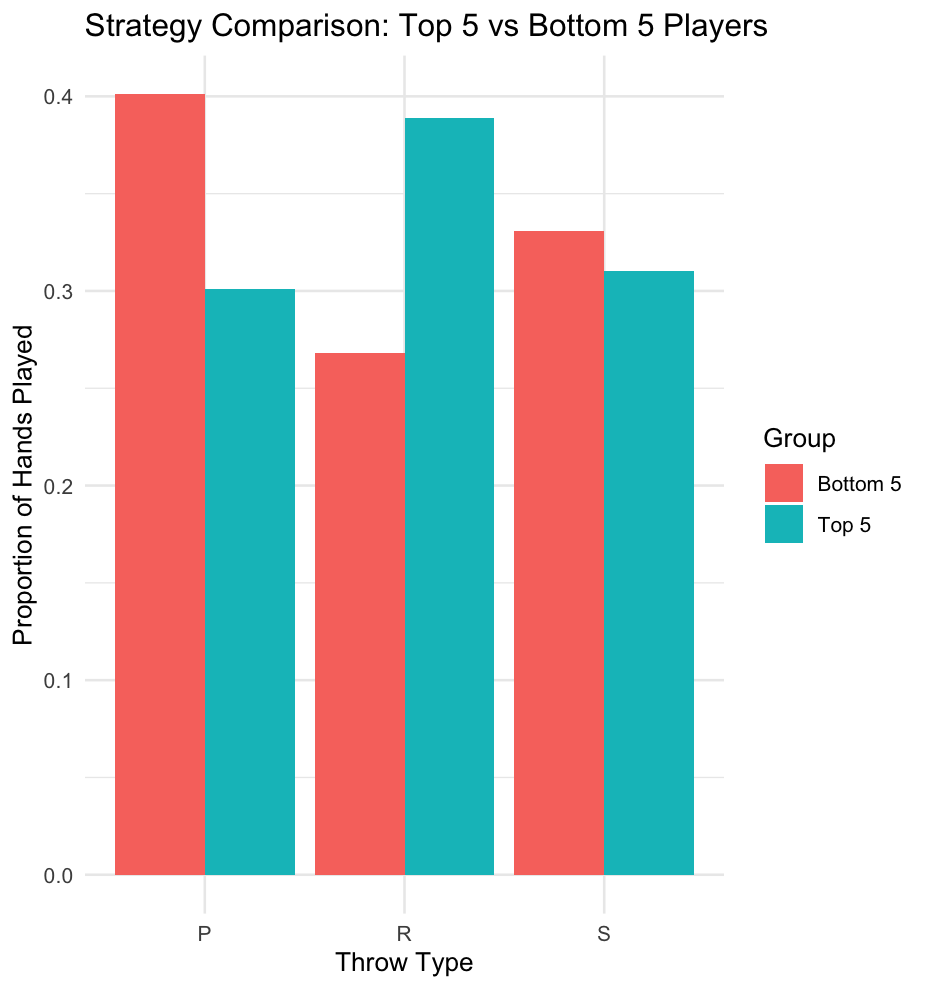
\includegraphics[width=0.75\textwidth]{figures/Strategy_Comparison_T5vB5.png}
\caption{Hand Selection Proportions by Group: Top 5 vs Bottom 5 Players}
\label{fig:strategy_comparison_T5vB5}
\end{figure}

This imbalance may have made the bottom five more predictable or less effective, especially if opponents adapted by countering with Scissors. On the other hand, the top five’s preference for Rock might have allowed them to win more encounters against players who overused Scissors or Paper. These contrasting patterns highlight how throw distribution is not just a matter of randomness but can reflect broader behavioral tendencies with measurable consequences in competitive outcomes.

We also analyzed results from the first two rounds of each game. Early rounds are critical because they offer an opportunity to set the tone and momentum for the rest of the game. As shown in Table~\ref{tab:first2_outcomes_t5b5}, top players won 99 early rounds while losing only 62. In contrast, the bottom five players only managed 61 early-round wins and lost 100 rounds. Draw rates were equal across both groups (69). These results are depicted graphically in below.

\begin{figure}[H]
\centering
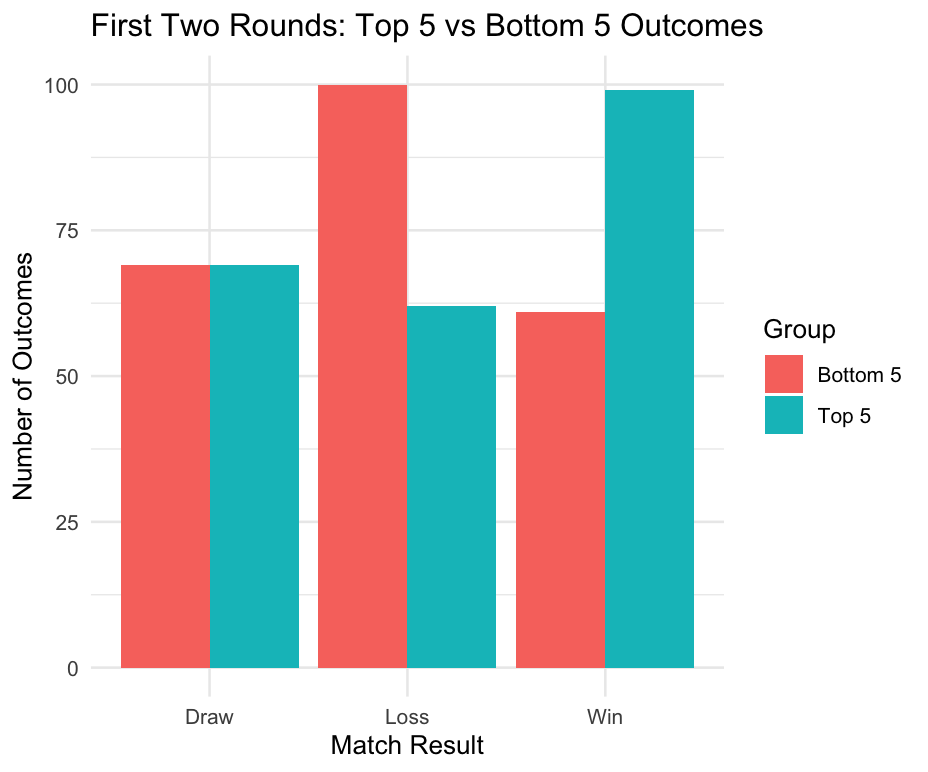
\includegraphics[width=0.75\textwidth]{figures/first2rounds_T5vB5.png}
\caption{Match Outcomes in First Two Rounds: Top 5 vs Bottom 5 Players}
\label{fig:first2rounds_T5vB5}
\end{figure}

Figure~\ref{fig:first2rounds_T5vB5} compares the outcomes of the first two rounds in each game for the top five and bottom five players. The differences are stark: the top five players secured 99 wins while only losing 62 early rounds. Meanwhile, the bottom five managed just 61 wins and suffered 100 losses in those same initial rounds. Draws were evenly distributed at 69 for each group.

This figure reinforces the importance of early momentum. Top players not only gained an edge in the opening stages but sustained this advantage through to final victory. In contrast, the bottom five players fell behind early and were unable to recover. This makes sense because the average number of matches per game across the entire tournament was \textbf{5.93}. These findings suggest that early-round performance may be a leading indicator of game outcomes, possibly due to psychological momentum, confidence, or the tactical advantage of playing from ahead. In other words, players who established early leads were more likely to convert those into full game wins. The bottom five players not only lost more early rounds but also showed overreliance on Paper—a possible liability if opponents adjusted with a Scissors-heavy strategy.

\subsection*{Conclusions}
\addcontentsline{toc}{subsection}{Conclusions}

Our findings offer three primary insights. First, strategic hand selection differs substantially between high- and low-performing players, with top players showing greater use of Rock and less use of Paper. Second, early-round dominance strongly correlates with final standings—suggesting that getting ahead early is a key to success. Third, the lack of statistically significant strategic shifts among most of our groupmates (except Isabel) points to consistent but potentially predictable strategies that may not be optimal in dynamic, adaptive settings.

While our analysis reveals strong patterns, it is limited in several ways. We did not control for the specific matchups players faced or whether they were reacting to an opponent’s known tendencies. Additionally, strategy shifts were only tested between two broad segments of the game (first two rounds vs. remaining rounds), and more granular time-series methods could reveal finer adaptation patterns. 

Despite these limitations, the tables and visualizations provide compelling evidence that strategic flexibility, early-round success, and balanced hand usage contribute to superior performance in Rock-Paper-Scissors tournaments.

% Optional GitHub reference (if allowed)
% For full code, visualizations, and data: \href{https://github.com/YOUR_REPO_HERE}{GitHub Repository}

\newpage

% Part 4
\section*{Part 4: Independent Exploration and Reflection}
\addcontentsline{toc}{section}{Part 4: Independent Exploration and Reflection}

\subsection*{Research Question and Motivation}
\addcontentsline{toc}{subsection}{Research Question and Motivation}

In this section, we explore the question: \textit{“What is the likelihood that a player will throw Rock, Paper, or Scissors based on what happened in the last round?”} Our interest stems from a behavioral economics perspective—specifically, whether players' choices can be predicted based on the outcome and decisions in the previous round. Understanding this could help characterize adaptive vs. non-adaptive strategies.

\subsection*{Methodology and Model Derivation}
\addcontentsline{toc}{subsection}{Methodology and Model Derivation}

As a forword, our codebase is maintained through \href{https://github.com/adelatorre2/adelatorre2-competition-group-project-mt220}{GitHub} and Git version control tools \cite{noauthor_git_nodate}. We first reformatted the tournament dataset into a long panel structure where each row represents a single player's throw per match, paired with their opponent's corresponding throw. We generated lag variables for each row: the player's previous throw, the opponent's previous throw, and the previous round's result (Win, Loss, Draw).

To model throw decision-making, we employed a multinomial logistic regression. Let $Y_i$ be the categorical variable representing player $i$'s current throw, taking one of three values: Rock ($R$), Paper ($P$), or Scissors ($S$). Using Rock as the baseline category, the model estimates the log-odds of throwing $P$ or $S$ relative to $R$:

\begin{align*}
\log\left(\frac{P(Y_i = P)}{P(Y_i = R)}\right) &= \beta_{0}^{(P)} + \boldsymbol{\beta}^{(P)} \cdot \mathbf{x}_i \\
\log\left(\frac{P(Y_i = S)}{P(Y_i = R)}\right) &= \beta_{0}^{(S)} + \boldsymbol{\beta}^{(S)} \cdot \mathbf{x}_i
\end{align*}

where $\mathbf{x}_i$ includes:
\begin{itemize}
  \item \texttt{Previous\_Throw}$_i$: the player's own throw in the previous round
  \item \texttt{Previous\_Opponent\_Throw}$_i$: their opponent's previous throw
  \item \texttt{Previous\_Result}$_i$: outcome of the previous round (Win/Loss/Draw)
\end{itemize}

The model was fitted using the \texttt{multinom()} function from the \texttt{nnet} package. The log-likelihood is maximized over the dataset $\{(y_i, \mathbf{x}_i)\}_{i=1}^{n}$:

\[
\ell(\boldsymbol{\theta}) = \sum_{i=1}^{n} \sum_{k \in \{P,S\}} \mathbb{1}_{\{y_i = k\}} \log\left(\frac{e^{\beta_0^{(k)} + \boldsymbol{\beta}^{(k)} \cdot \mathbf{x}_i}}{1 + \sum_{j \in \{P,S\}} e^{\beta_0^{(j)} + \boldsymbol{\beta}^{(j)} \cdot \mathbf{x}_i}}\right)
\]

\subsection*{Key Findings}
\addcontentsline{toc}{subsection}{Key Findings}

After fitting the model, we used the estimated coefficients to compute predicted probabilities for each throw type conditional on the result of the previous round. These were visualized in Figure~\ref{fig:pred_probs}.

\begin{figure}[H]
  \centering
  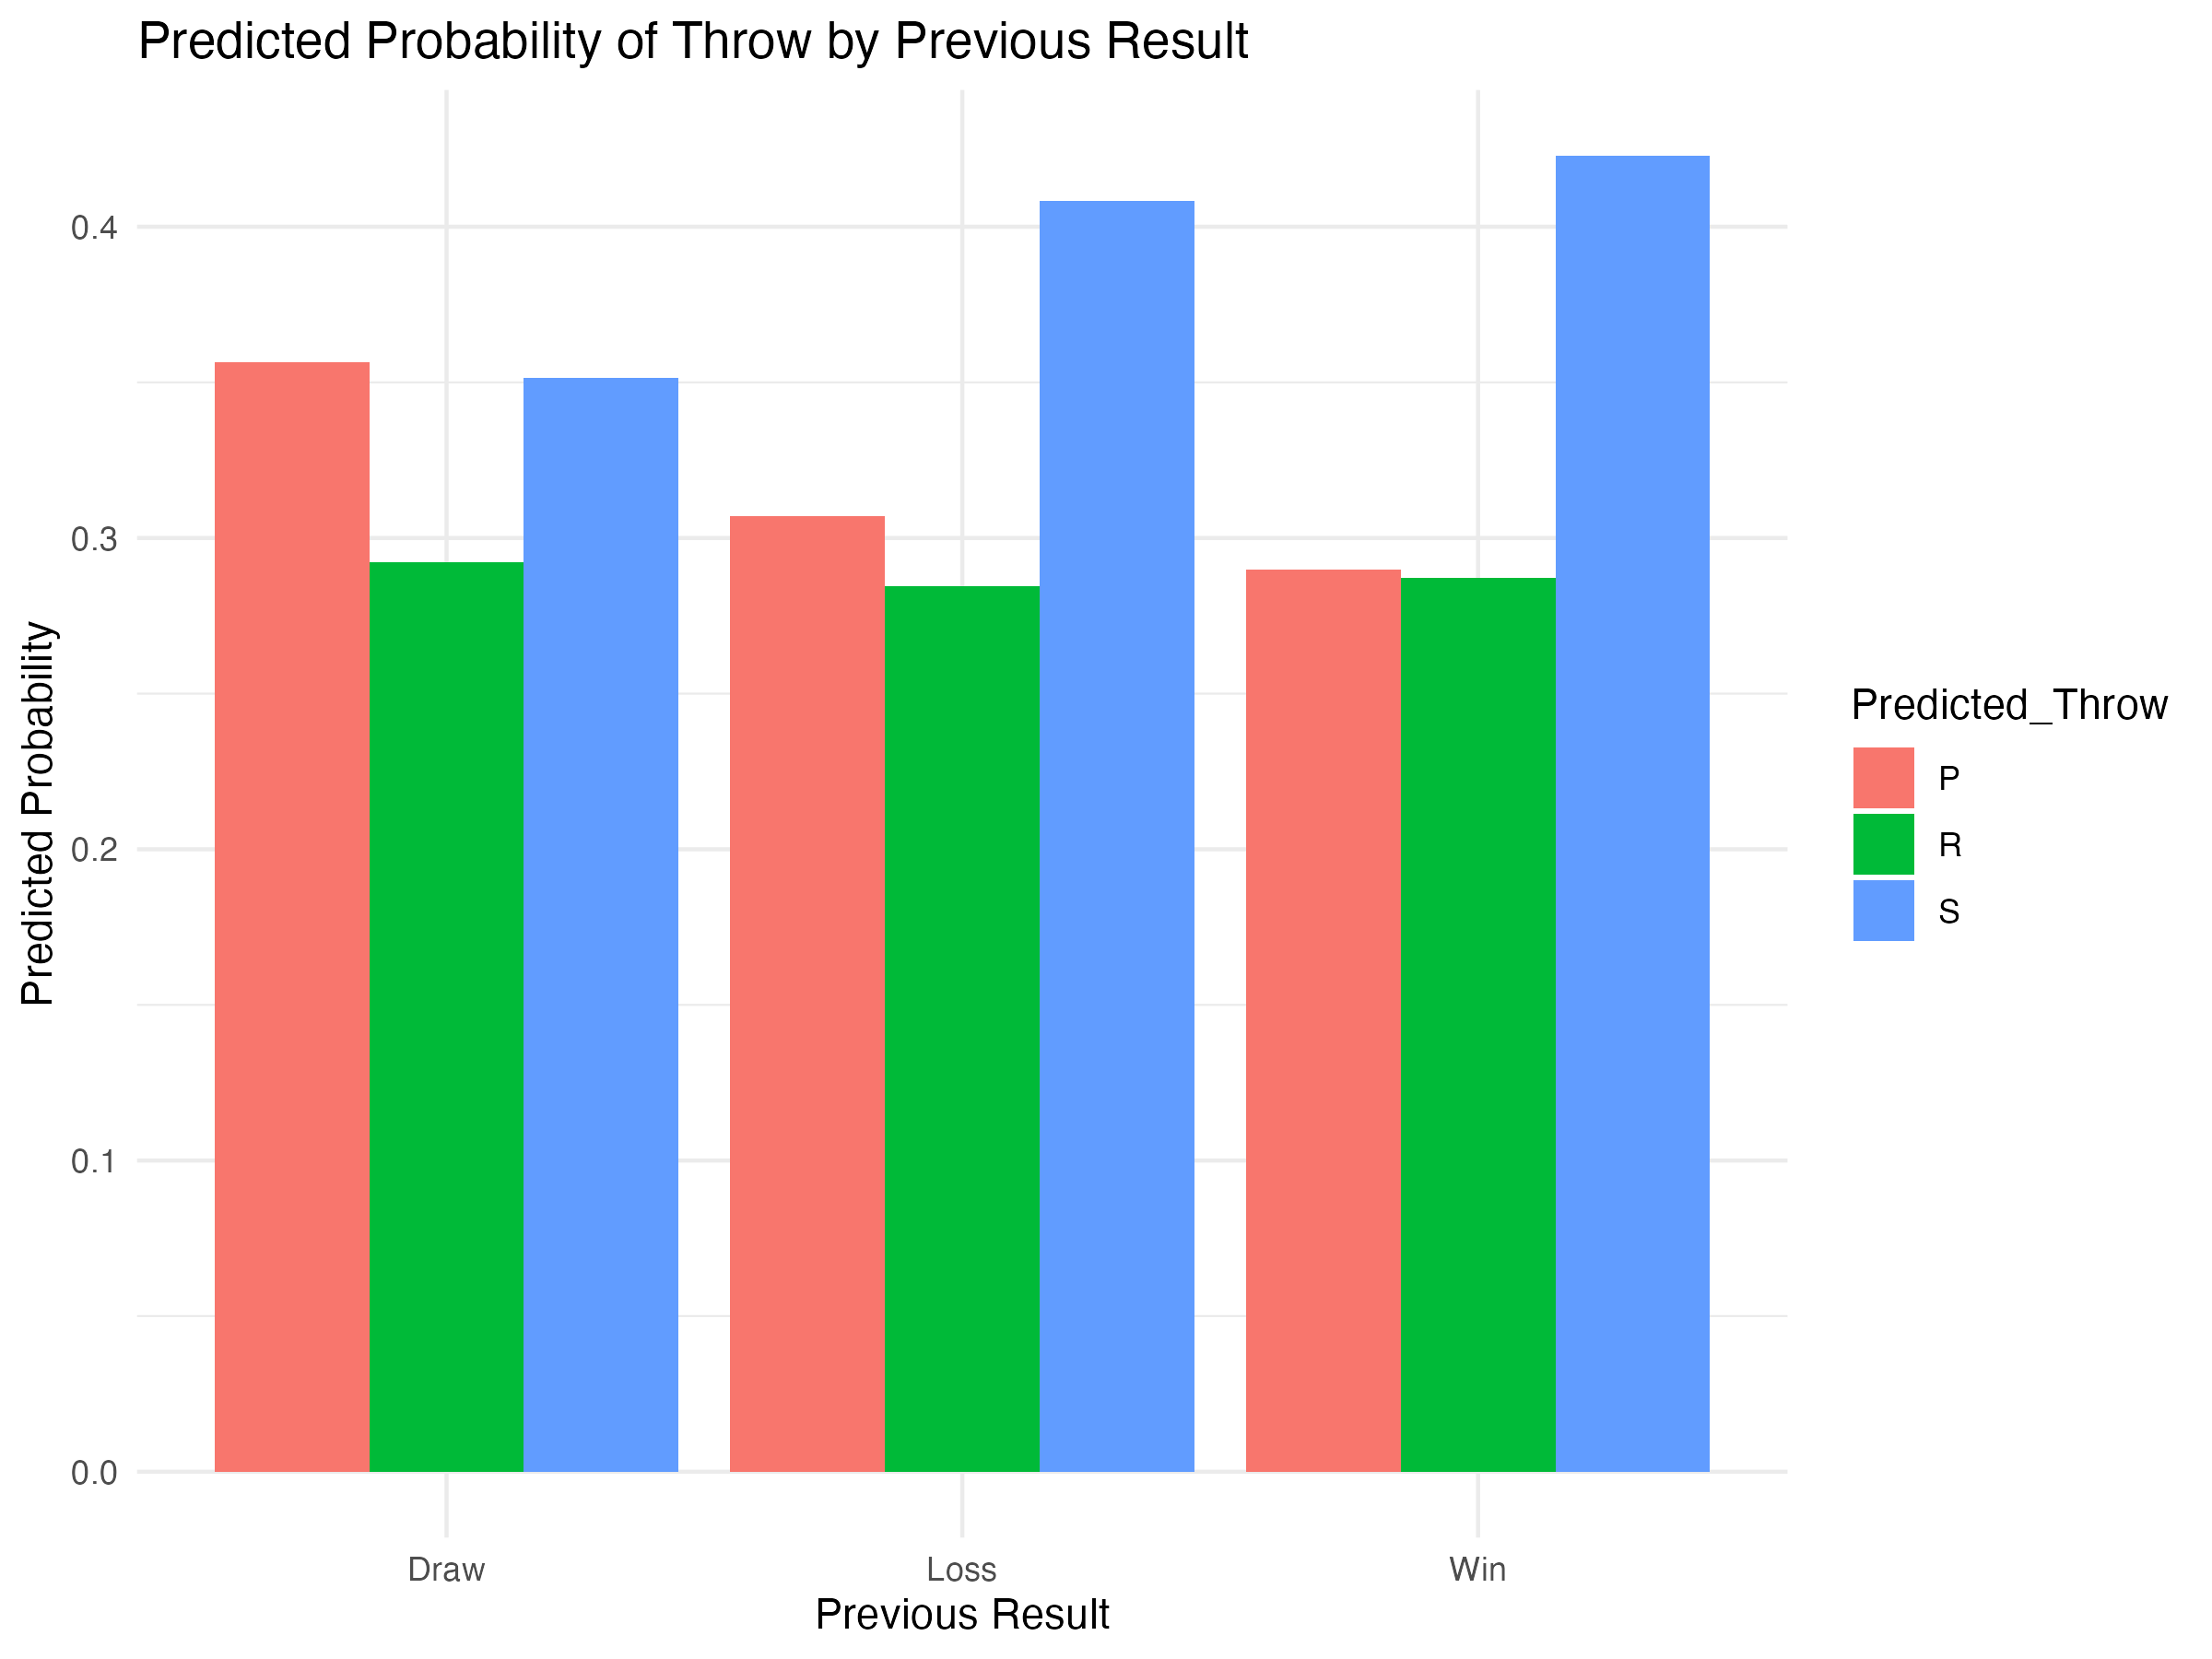
\includegraphics[width=0.8\linewidth]{figures/predicted_throw_probabilities_by_result.png}
  \caption{Predicted Probabilities of Throw Type by Previous Round Result}
  \label{fig:pred_probs}
\end{figure}

The visualization reveals strategic asymmetries: after a \textbf{win}, players are most likely to throw \textbf{Rock}, suggesting potential stickiness or overconfidence in that strategy. After a \textbf{loss}, players are also more likely to switch to Rock, possibly due to an adjustment attempt. After a \textbf{draw}, the distribution is more balanced, with a slight tilt toward Paper. Coefficient tables (see Appendix~\ref{tab:model_coefficients_part4}) show that the previous opponent’s throw has a relatively large effect size in determining the player's next move. For example, a previous opponent throw of Rock increases the odds of the player choosing Paper significantly.

\subsection*{Limitations}
\addcontentsline{toc}{subsection}{Limitations}

While our findings are suggestive, several caveats must be acknowledged. We do not control for the identity of the opponent or within-game dynamics beyond lag-1 behavior, which may introduce omitted variable bias. The multinomial model assumes the independence of irrelevant alternatives (IIA), which may not hold in behavioral settings where decision-making is context-dependent. Early rounds without lagged context were excluded, potentially biasing the sample toward longer games or more experienced players. Finally, the model does not account for strategy evolution over time, which suggests the need for more dynamic models like Markov Switching or Hidden Markov Models in future analyses.

\subsection*{Future Directions}
\addcontentsline{toc}{subsection}{Future Directions}

Building on this work, future iterations of the project could explore heterogeneity in strategy by player using mixed-effects multinomial models. Further comparisons could be made between high-performing players and others to examine divergent strategies. Additionally, incorporating round number or game ID as fixed effects could help capture learning or fatigue effects. Modeling the opponent’s behavior as a separate, interactive process would also help account for joint strategic dynamics and feedback loops between players.

\subsection*{Conclusion}
\addcontentsline{toc}{subsection}{Conclusion}

Using a multinomial logistic model, we found that prior outcomes and player/opponent throw history significantly influence the likelihood of selecting a throw in a Rock-Paper-Scissors tournament. The results point to a modest tendency to favor Rock following both wins and losses—suggesting cognitive biases or adaptation heuristics. This framework can be extended to richer models of decision-making and has potential applications in understanding sequential strategic behavior in low-stakes competitive games.

\newpage
\section*{Appendix: Part 1 Tables}
\addcontentsline{toc}{section}{Appendix: Part 1 Tables}

\begin{table}[H]
\centering
\caption{Theoretical Probabilities for Hand Matchups}
\label{tab:theoretical_matrix}
\begin{tabular}{lccc}
\toprule
\textbf{Player 1 vs Player 2} & \textbf{Rock} & \textbf{Paper} & \textbf{Scissors} \\
\midrule
Rock     & 0.111 & 0.111 & 0.111 \\
Paper    & 0.111 & 0.111 & 0.111 \\
Scissors & 0.111 & 0.111 & 0.111 \\
\bottomrule
\end{tabular}
\end{table}

\begin{table}[H]
\centering
\caption{Empirical Matchup Counts from Data}
\label{tab:empirical_counts}
\begin{tabular}{lccc}
\toprule
\textbf{Player 1 vs Player 2} & \textbf{Rock} & \textbf{Paper} & \textbf{Scissors} \\
\midrule
Rock     & 110 & 169 & 199 \\
Paper    & 152 & 151 & 190 \\
Scissors & 198 & 218 & 244 \\
\bottomrule
\end{tabular}
\end{table}

\begin{table}[H]
\centering
\caption{Empirical Matchup Proportions (Rounded to 3 Decimals)}
\label{tab:empirical_proportions}
\begin{tabular}{lccc}
\toprule
\textbf{Player 1 vs Player 2} & \textbf{Rock} & \textbf{Paper} & \textbf{Scissors} \\
\midrule
Rock     & 0.067 & 0.104 & 0.122 \\
Paper    & 0.093 & 0.093 & 0.116 \\
Scissors & 0.121 & 0.134 & 0.150 \\
\bottomrule
\end{tabular}
\end{table}

\newpage
\appendix
\section*{Appendix: Part 2 Tables}
\addcontentsline{toc}{section}{Appendix: Part 2 Tables}

\begin{multicols}{2}

\begin{table}[H]
\centering
\caption{Overall Throw Counts}
\label{tab:overall_counts}
\begin{tabular}{lrrr}
\toprule
\textbf{Player} & \textbf{R} & \textbf{P} & \textbf{S} \\
\midrule
julia & 59 & 39 & 26 \\
lilly & 2 & 35 & 75 \\
leah & 22 & 49 & 71 \\
ellie & 28 & 49 & 74 \\
isabel & 50 & 28 & 61 \\
meredith & 43 & 53 & 44 \\
brooklyn & 36 & 21 & 71 \\
lindsey & 36 & 13 & 88 \\
brian & 32 & 35 & 60 \\
bruno & 31 & 69 & 49 \\
alejandro & 21 & 39 & 77 \\
matt & 46 & 36 & 44 \\
arvind & 57 & 30 & 42 \\
james & 42 & 35 & 70 \\
neev & 53 & 36 & 30 \\
hayden & 76 & 72 & 8 \\
devin & 44 & 57 & 35 \\
olivia & 44 & 49 & 71 \\
molly & 31 & 61 & 40 \\
ryan & 13 & 42 & 91 \\
john & 27 & 57 & 61 \\
\bottomrule
\end{tabular}
\end{table}

\begin{table}[H]
\centering
\caption{First Two Rounds – Throw Counts}
\label{tab:first2_counts}
\begin{tabular}{lrrr}
\toprule
\textbf{Player} & \textbf{R} & \textbf{P} & \textbf{S} \\
\midrule
julia & 29 & 10 & 7 \\
lilly & 1 & 14 & 29 \\
leah & 5 & 17 & 24 \\
ellie & 4 & 10 & 30 \\
isabel & 19 & 3 & 24 \\
meredith & 12 & 14 & 20 \\
brooklyn & 8 & 4 & 34 \\
lindsey & 13 & 1 & 30 \\
brian & 12 & 10 & 24 \\
bruno & 7 & 22 & 17 \\
alejandro & 6 & 12 & 28 \\
matt & 18 & 9 & 19 \\
arvind & 20 & 7 & 19 \\
james & 17 & 5 & 24 \\
neev & 23 & 16 & 7 \\
hayden & 31 & 13 & 2 \\
devin & 14 & 20 & 12 \\
olivia & 10 & 10 & 26 \\
molly & 10 & 23 & 13 \\
ryan & 1 & 9 & 36 \\
john & 5 & 22 & 28 \\
\bottomrule
\end{tabular}
\end{table}

\begin{table}[H]
\centering
\caption{Remaining Rounds – Throw Counts}
\label{tab:rest_counts}
\begin{tabular}{lrrr}
\toprule
\textbf{Player} & \textbf{R} & \textbf{P} & \textbf{S} \\
\midrule
julia & 30 & 29 & 19 \\
lilly & 1 & 21 & 46 \\
leah & 17 & 32 & 47 \\
ellie & 24 & 39 & 44 \\
isabel & 31 & 25 & 37 \\
meredith & 31 & 39 & 24 \\
brooklyn & 28 & 17 & 37 \\
lindsey & 23 & 12 & 58 \\
brian & 20 & 25 & 36 \\
bruno & 24 & 47 & 32 \\
alejandro & 15 & 27 & 49 \\
matt & 28 & 27 & 25 \\
arvind & 37 & 23 & 23 \\
james & 25 & 30 & 46 \\
neev & 30 & 20 & 23 \\
hayden & 45 & 59 & 6 \\
devin & 30 & 37 & 23 \\
olivia & 34 & 39 & 45 \\
molly & 21 & 38 & 27 \\
ryan & 12 & 33 & 55 \\
john & 22 & 35 & 33 \\
\bottomrule
\end{tabular}
\end{table}

\begin{table}[H]
\centering
\caption{First Two Rounds – Outcomes}
\label{tab:first2_outcomes}
\begin{tabular}{lrrr}
\toprule
\textbf{Player} & \textbf{Win} & \textbf{Loss} & \textbf{Draw} \\
\midrule
julia & 29 & 5 & 12 \\
lilly & 9 & 18 & 17 \\
leah & 12 & 18 & 16 \\
ellie & 13 & 15 & 16 \\
isabel & 17 & 11 & 18 \\
meredith & 17 & 12 & 17 \\
brooklyn & 11 & 16 & 19 \\
lindsey & 11 & 16 & 17 \\
brian & 15 & 15 & 16 \\
bruno & 12 & 18 & 16 \\
alejandro & 13 & 17 & 16 \\
matt & 27 & 12 & 7 \\
arvind & 21 & 14 & 11 \\
james & 15 & 14 & 17 \\
neev & 22 & 14 & 10 \\
hayden & 18 & 11 & 17 \\
devin & 13 & 25 & 8 \\
olivia & 20 & 13 & 13 \\
molly & 12 & 24 & 10 \\
ryan & 6 & 14 & 26 \\
john & 9 & 16 & 21 \\
\bottomrule
\end{tabular}
\end{table}

\begin{table}[H]
\centering
\caption{Remaining Rounds – Outcomes}
\label{tab:rest_outcomes}
\begin{tabular}{lrrr}
\toprule
\textbf{Player} & \textbf{Win} & \textbf{Loss} & \textbf{Draw} \\
\midrule
julia & 25 & 34 & 19 \\
lilly & 25 & 27 & 16 \\
leah & 29 & 29 & 38 \\
ellie & 33 & 34 & 40 \\
isabel & 37 & 28 & 28 \\
meredith & 25 & 40 & 29 \\
brooklyn & 30 & 37 & 15 \\
lindsey & 28 & 31 & 34 \\
brian & 36 & 28 & 17 \\
bruno & 31 & 36 & 36 \\
alejandro & 32 & 39 & 20 \\
matt & 30 & 29 & 21 \\
arvind & 30 & 28 & 25 \\
james & 38 & 29 & 34 \\
neev & 32 & 21 & 20 \\
hayden & 38 & 34 & 38 \\
devin & 29 & 32 & 28 \\
olivia & 33 & 35 & 30 \\
molly & 29 & 37 & 20 \\
ryan & 25 & 36 & 39 \\
john & 30 & 35 & 25 \\
\bottomrule
\end{tabular}
\end{table}

\newpage
\begin{table}[H]
\centering
\caption{Chi-Square Test Results for Strategy Shift Between Game Segments}
\label{tab:strategy_shift}
\begin{tabular}{lrrl}
\toprule
\textbf{Player} & \textbf{p-value} & \textbf{Chi-Square Stat} & \textbf{Significant} \\
\midrule
julia     & 0.0299 & 7.021 & Yes \\
lilly     & 0.9437 & 0.116 & No \\
leah      & 0.5708 & 1.121 & No \\
ellie     & 0.0088 & 9.459 & Yes \\
isabel    & 0.0187 & 7.953 & Yes \\
meredith  & 0.0983 & 4.640 & No \\
brooklyn  & 0.0069 & 9.947 & Yes \\
lindsey   & 0.1368 & 3.978 & No \\
brian     & 0.5273 & 1.280 & No \\
bruno     & 0.5048 & 1.367 & No \\
alejandro & 0.7255 & 0.642 & No \\
matt      & 0.2188 & 3.039 & No \\
arvind    & 0.1593 & 3.674 & No \\
james     & 0.0360 & 6.648 & Yes \\
neev      & 0.1366 & 3.986 & No \\
hayden    & 0.0024 & 12.179 & Yes \\
devin     & 0.0316 & 6.850 & Yes \\
olivia    & 0.0013 & 13.165 & Yes \\
molly     & 0.3433 & 2.140 & No \\
ryan      & 0.0283 & 7.178 & Yes \\
john      & 0.3119 & 2.319 & No \\
\bottomrule
\end{tabular}
\end{table}

\end{multicols}


% Center the graph, without the multicol environment
\begin{figure}[H]
\centering
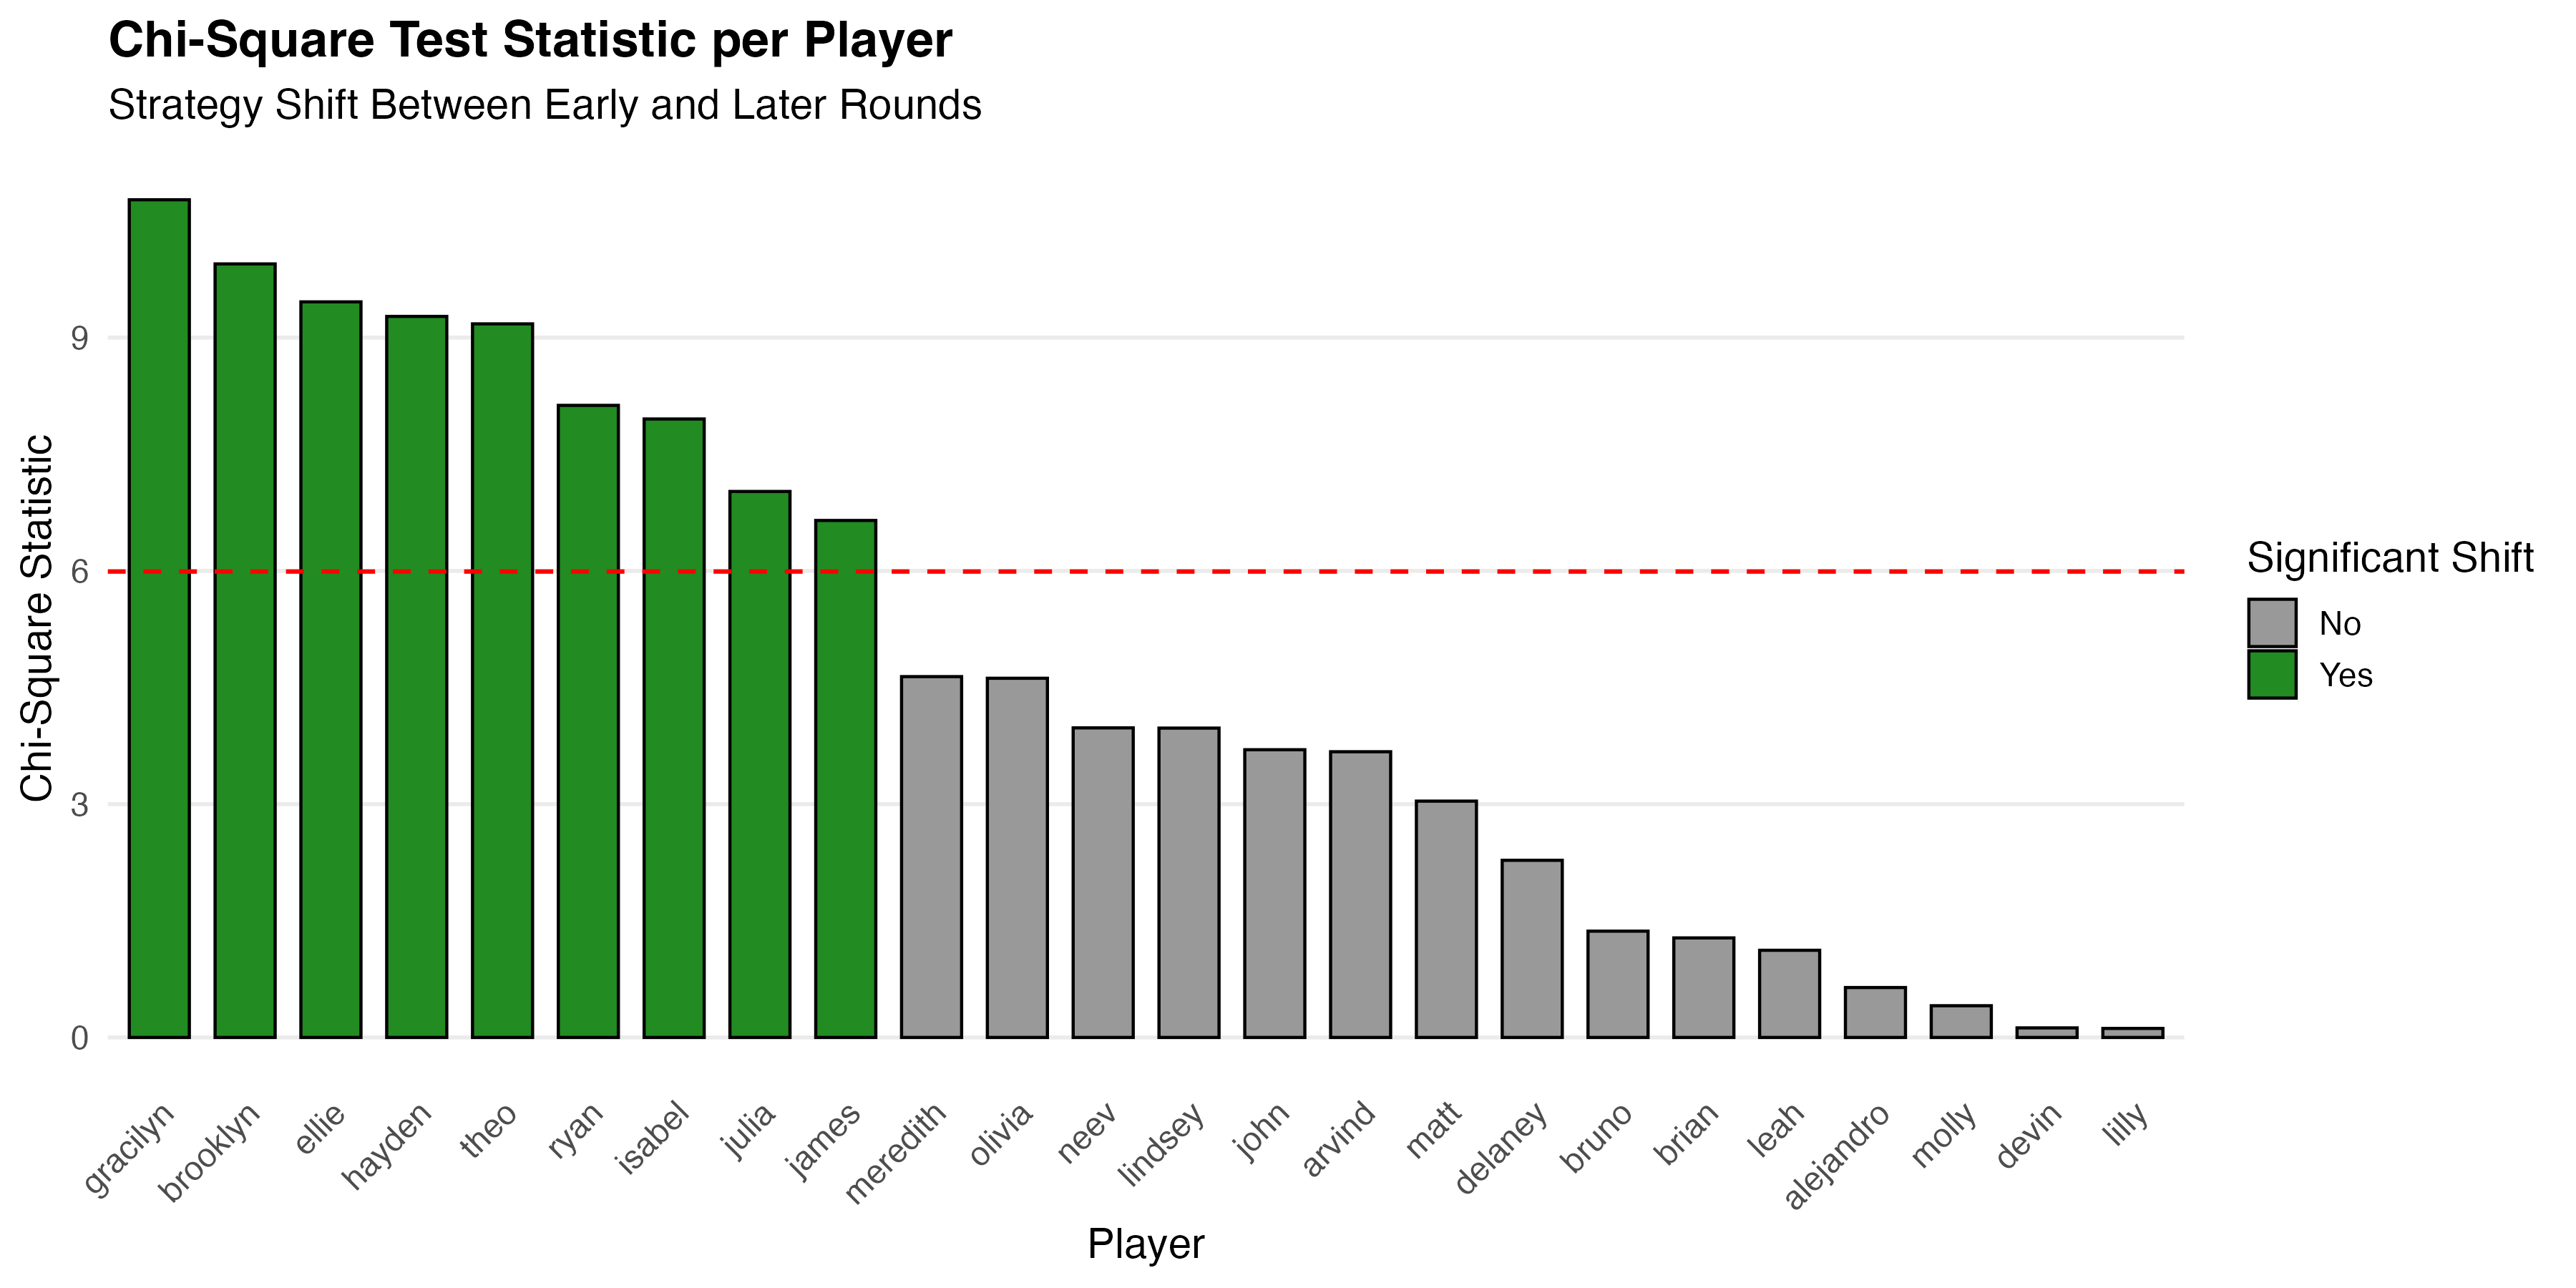
\includegraphics[width=0.9\textwidth]{figures/strategy_shift_chisq.png}
\caption{Chi-Square Test Statistic per Player: Strategy Shift Between Early and Later Rounds. Bars above the red dashed line indicate statistically significant changes (p < 0.05).}
\label{fig:strategy_shift_bar_appendix}
\end{figure}

\newpage
\section*{Appendix: Part 3 Tables}
\addcontentsline{toc}{section}{Appendix: Part 3 Tables}

\begin{table}[H]
\centering
\caption{Total Individual Match Results by Player}
\label{tab:total_match_results}
\begin{tabular}{lrrr}
\toprule
\textbf{Player} & \textbf{Match Wins} & \textbf{Match Losses} & \textbf{Match Draws} \\
\midrule
matt      & 57 & 41 & 28 \\
hayden    & 56 & 45 & 55 \\
theo      & 55 & 45 & 28 \\
neev      & 54 & 35 & 30 \\
isabel    & 54 & 37 & 46 \\
julia     & 54 & 39 & 31 \\
james     & 53 & 42 & 51 \\
gracilyn  & 53 & 46 & 30 \\
arvind    & 51 & 42 & 36 \\
brian     & 50 & 43 & 33 \\
ryan      & 50 & 43 & 53 \\
ellie     & 46 & 49 & 56 \\
alejandro & 44 & 56 & 36 \\
delaney   & 43 & 46 & 46 \\
olivia    & 43 & 56 & 65 \\
meredith  & 42 & 52 & 46 \\
devin     & 42 & 54 & 37 \\
john      & 41 & 43 & 45 \\
leah      & 41 & 47 & 54 \\
brooklyn  & 41 & 53 & 34 \\
bruno     & 41 & 53 & 52 \\
lindsey   & 38 & 47 & 51 \\
molly     & 36 & 60 & 34 \\
lilly     & 34 & 45 & 33 \\
\bottomrule
\end{tabular}
\end{table}

\begin{table}
\centering
\caption{Total Games Won and Lost by Player with Tournament Rank}
\label{tab:total_game_results}
\begin{tabular}{lrrr}
\toprule
\textbf{Player} & \textbf{Game Wins} & \textbf{Game Losses} & \textbf{Rank} \\
\midrule
neev      & 16 & 7 & 1 \\
isabel    & 15 & 8 & 2 \\
matt      & 14 & 9 & 3 \\
james     & 14 & 9 & 3 \\
hayden    & 14 & 9 & 3 \\
theo      & 14 & 9 & 3 \\
julia     & 13 & 10 & 4 \\
brian     & 13 & 10 & 4 \\
ryan      & 13 & 10 & 4 \\
gracilyn  & 13 & 10 & 4 \\
arvind    & 12 & 11 & 5 \\
john      & 11 & 11 & 6 \\
lilly     & 10 & 12 & 7 \\
lindsey   & 10 & 12 & 7 \\
leah      & 10 & 13 & 8 \\
brooklyn  & 10 & 13 & 8 \\
alejandro & 10 & 13 & 8 \\
delaney   & 10 & 13 & 8 \\
ellie     & 9  & 13 & 9 \\
meredith  & 9  & 14 & 10 \\
bruno     & 9  & 14 & 10 \\
devin     & 9  & 14 & 10 \\
olivia    & 9  & 14 & 10 \\
molly     & 7  & 16 & 11 \\
\bottomrule
\end{tabular}
\end{table}

\begin{table}[H]
\centering
\tiny
\caption{Groupmate Strategy Summary and Tournament Results}
\label{tab:groupmate_summary}
\begin{tabularx}{\textwidth}{lrrr>{\centering\arraybackslash}X rrr rrr >{\centering\arraybackslash}X}
\toprule
\textbf{Player} & \textbf{Game Wins} & \textbf{Game Losses} & \textbf{Rank} & \makecell{\textbf{Most}\\\textbf{Used}\\\textbf{Throw}} &
\makecell{\textbf{First}\\\textbf{Win}} & \makecell{\textbf{First}\\\textbf{Loss}} & \makecell{\textbf{First}\\\textbf{Draw}} &
\makecell{\textbf{Rest}\\\textbf{Win}} & \makecell{\textbf{Rest}\\\textbf{Loss}} & \makecell{\textbf{Rest}\\\textbf{Draw}} &
\makecell{\textbf{Significant}\\\textbf{Shift?}} \\
\midrule
isabel     & 15 & 8  & 2  & S & 17 & 11 & 18 & 37 & 28 & 28 & Yes \\
matt       & 14 & 9  & 3  & R & 27 & 12 &  7 & 30 & 29 & 21 & No  \\
brian      & 13 & 10 & 4  & S & 15 & 15 & 16 & 36 & 28 & 17 & No  \\
alejandro  & 10 & 13 & 8  & S & 13 & 17 & 16 & 32 & 39 & 20 & No  \\
meredith   & 9  & 14 & 10 & P & 17 & 12 & 17 & 25 & 40 & 29 & No  \\
\bottomrule
\end{tabularx}
\end{table}

\begin{table}[H]
\centering
\small
\caption{Hand Usage Proportions: Top 5 vs Bottom 5 Players}
\label{tab:top5_vs_bottom5_strategy}
\begin{tabular}{lccc}
\toprule
\textbf{Group} & \textbf{Proportion Rock} & \textbf{Proportion Paper} & \textbf{Proportion Scissors} \\
\midrule
Top 5     & 0.389 & 0.301 & 0.310 \\
Bottom 5  & 0.268 & 0.401 & 0.331 \\
\bottomrule
\end{tabular}
\end{table}

\begin{table}[H]
\centering
\small
\caption{Match Outcomes in First Two Rounds: Top 5 vs Bottom 5 Players}
\label{tab:first2_outcomes_t5b5}
\begin{tabular}{lll}
\toprule
\textbf{Group} & \textbf{Outcome} & \textbf{Count} \\
\midrule
Top 5     & Win  & 99 \\
Top 5     & Loss & 62 \\
Top 5     & Draw & 69 \\
Bottom 5  & Win  & 61 \\
Bottom 5  & Loss & 100 \\
Bottom 5  & Draw & 69 \\
\bottomrule
\end{tabular}
\end{table}

\newpage

\section*{Appendix: Part 4 Tables}
\addcontentsline{toc}{section}{Appendix: Part 4 Tables}

\begin{table}[H]
\centering

\caption{Estimated Coefficients from Multinomial Logistic Regression Model (Baseline = Rock)}
\label{tab:model_coefficients_part4}
\begin{tabular}{lrr}
\toprule
\textbf{Predictor} & \textbf{P vs R} & \textbf{S vs R} \\
\midrule
(Intercept) & -0.214992 & 0.093638 \\
Previous\_ThrowR & 0.083627 & -0.085216 \\
Previous\_ThrowS & 0.159360 & 0.081727 \\
Previous\_Opponent\_ThrowR & 0.635958 & 0.425529 \\
Previous\_Opponent\_ThrowS & 0.367453 & -0.032258 \\
Previous\_ResultLoss & -0.133348 & 0.139584 \\
Previous\_ResultWin & -0.172928 & 0.185359 \\
\bottomrule
\end{tabular}
\end{table}


% bibliography
\newpage
\phantomsection
\addcontentsline{toc}{section}{References}
\bibliographystyle{apalike}
\bibliography{references}   % APA-style citations (recommended for your type of paper)
% \bibliographystyle{plain}  % Numeric references [1], [2], etc.
% \bibliographystyle{ieeetr} % IEEE numeric format

\end{document}